\documentclass[../main.tex]{subfiles}
\begin{document}
\chapter{Architettura di certificazione cloud basata su sonde}
In questo capitolo verrà presentata un'architettura di certificazione per sistemi cloud basata sull'utilizzo di sonde, compatibile con il framework CUMULUS.
Le sonde sono definite come componenti software autonomi, scalabili e orientati all'esecuzione parallela e schedulata dei processi, di cui può essere effettuato il deployment a tutti i livelli dello stack cloud (\textit{IaaS}, \textit{PaaS} e \textit{SaaS}).

\`E possibile raggruppare le sonde in due categorie:
\begin{itemize}
\item \textit{Sonde di testing}: si occupano di eseguire dei casi di test, rappresentati da driver di sonda, sul sistema target, in base a una serie di input forniti. I risultati dei test vengono poi collezionati, organizzati, validati e utilizzati per effettuare il processo di certificazione.
\item \textit{Sonde di monitoraggio}: si occupano di effettuare monitoraggio attivo del servizio da testare, raccogliendo in modo temporizzato i dati relativi allo stato globale del sistema target. Essi vengono poi sanitizzati e aggregati affinché sia possibile dedurre le caratteristiche di un evento e utilizzarle per supportare il processo di certificazione.
\end{itemize}
\newpage
\section{Componenti della sonda di testing}
Nel progetto di tesi è stata realizzata una \textit{sonda di testing} ed è stata posizionata all'interno del framework CUMULUS.
Verranno ora illustrati i componenti principali della sonda descrivendo la corrispondenza degli stessi con i requisiti di CUMULUS.
\subsection{Communication Bus}
Il \textit{Communication Bus} rappresenta il protocollo di comunicazione tra il \textit{Test Manager} e le sonde (Figura \ref{fig:CommunicationSonda}).
Esso è realizzato mediante un meccanismo distribuito basato su code, nel quale il \textit{Test Manager} rappresenta il produttore e le sonde hanno il ruolo di consumatori.
Il canale è interamente gestito dal \textit{Test Manager}, che si occupa di creare le code e di configurare il controllo degli accessi per abilitarne l'utilizzo alle varie sonde.
Il Test Manager deposita sul canale i \textit{collector} da eseguire, le sonde eseguono i test specificati nei \textit{collector} con le configurazioni indicate, dopodiché restituiscono i risultati al Test Manager.
\begin{figure}[H]
\centering
\makebox[\textwidth]{
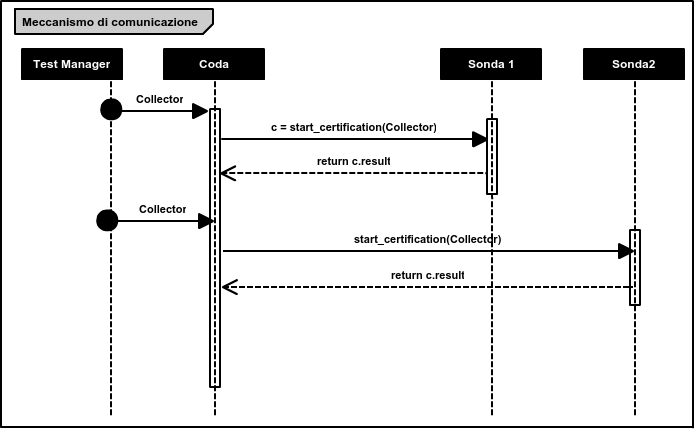
\includegraphics[width=\textwidth]{immagini/CommunicationSonda.png}
}
\caption{Meccanismo di comunicazione tra Test Manager e Sonda}\label{fig:CommunicationSonda}
\end{figure}
\newpage
\subsection {Subscription Service}
Il componente \textit{Subscription Service} è di fondamentale importanza: affinché sia possibile la comunicazione tra Test Manager e sonda, è necessario che quest'ultima conosca le informazioni per potersi connettere al \textit{Communication Bus} e iniziare così a consumare i \textit{Collector}.
Questo servizio consiste in un'interfaccia pubblica che permette di fornire alla sonda la configurazione per la sottoscrizione al canale di comunicazione.

In base alle informazioni fornite a questo servizio è possibile implementare varie topologie di \textit{deployment}.
\`E possibile, ad esempio, raggruppare le sonde in \textit{famiglie}, per consentire l'instradamento dei \textit{collector} relativi a un determinato \textit{ToT} a una specifico gruppo di sonde (Figura \ref{fig:Subscription}).
Solitamente il servizio viene invocato dal Test Manager (1)(2) nella fase di \textit{bootstrapping} della sonda, tuttavia le informazioni di \textit{Subscription} possono essere già state definite a priori tramite il file di configurazione (3) (\textit{/etc/testagent/subscription.conf}).
Solo a questo punto la sonda è in grado di effettuare la connessione al \textit{Communication Bus} e può effettuare l'iscrizione alla coda corrispondente alla propria famiglia.
Viene quindi avviato il \textit{Collector Dispatcher} e la sonda può iniziare a consumare i \textit{collector}.
\begin{figure}[H]
\centering
\makebox[\textwidth]{
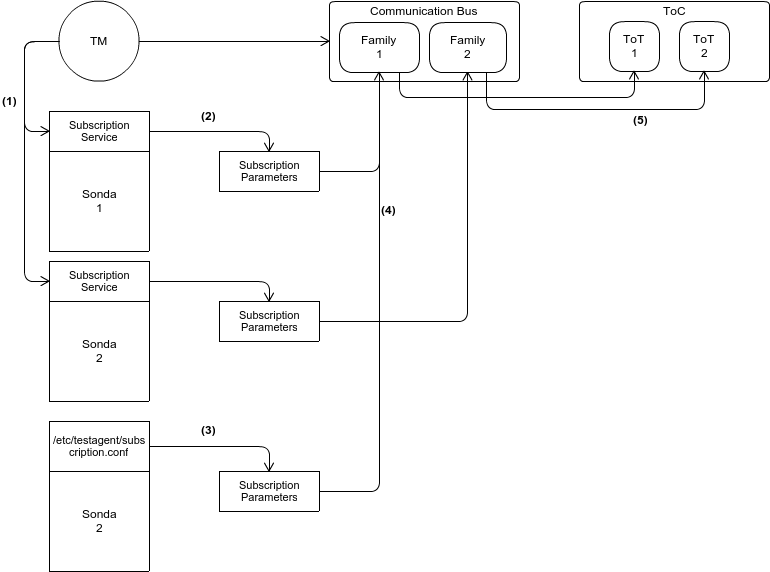
\includegraphics[width=\textwidth]{immagini/Subscription.png}
}
\caption{Meccanismo di sottoscrizione della sonda al canale di comunicazione}\label{fig:Subscription}
\end{figure}

\subsection {Collector Dispatcher}
Questo componente effettua il \textit{dispatching} dei \textit{Collector} su più processi, al fine di parallelizzarne l'esecuzione e sfruttare al meglio le caratteristiche di \textit{multithreading} implementate a livello hardware e/o di hypervisor sulla macchina che ospita la sonda.
Ogni qualvolta un \textit{Collector} viene ricevuto da una sonda ne viene effettuato il parsing, dopodiché viene avviato un sottoprocesso che effettua l'esecuzione serializzata di tutti i \textit{TestCase} descritti nel Collector e il driver di sonda specificato dallo stesso. Successivamente all'esecuzione dell'ultimo TestCase, viene invocato il \textit{Results Collector}.

\subsection {XML Parser \& Marshaller}
L'\textit{XML Parser \& Marshaller} è il componente che si occupa di effettuare il parsing dei messaggi e realizza le strutture dati contenenti le informazioni da utilizzare ai fini dell'esecuzione dei \textit{collector}.
Il funzionamento di questo componente è mostrato in figura \ref{fig:XMLParser}.
Il Test Manager effettua il parsing del \textit{Certification Model} deposita i singoli \textit{Collector} sulla coda, indicando l'\textit{ID} del \textit{Certification Model} nell'attributo \textit{cm\_id}. La sonda, alla ricezione del \textit{Collector} (1), ne effettua il parsing. Procede poi con il parsing dei \textit{TestCases} (2), dei \textit{TestInstance} (3) e dei dati in \textit{Input} (3).
Per ogni elemento di cui è stato effettuato il parsing viene allocata la struttura dati corrispondente (5)(6)(7)(8).
Tutte le strutture dati vengono poi aggregate in modo gerarchico sotto l'unico elemento radice \textit{Collector}(9)(10)(11).
Questo viene poi inoltrato al \textit{Probe Wrapper} per l'esecuzione dei casi di test(12).
\begin{figure}[H]
\centering
\makebox[\textwidth]{
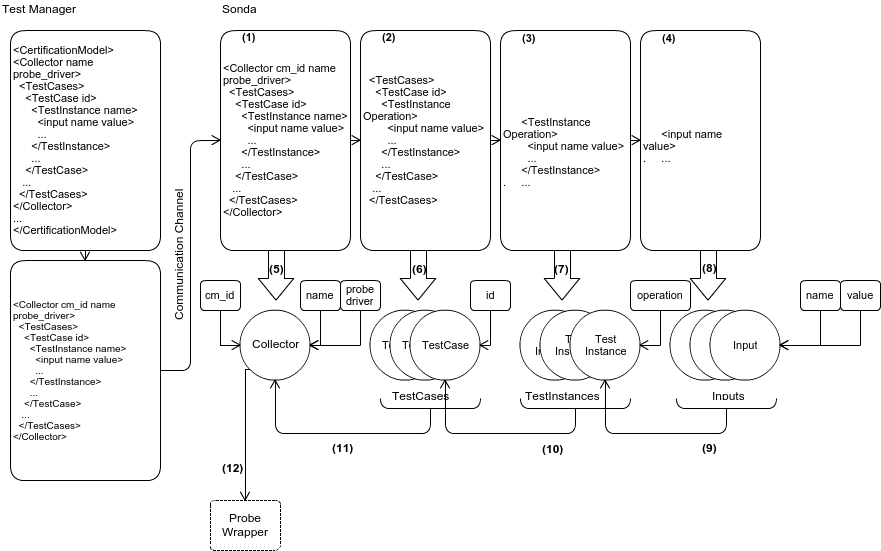
\includegraphics[width=\textwidth]{immagini/XMLParser.png}
}
\caption{XML Parser \& Marshaller}\label{fig:XMLParser}
\end{figure}

\newpage
\subsection {Self Assessment module}
Il \textit{Self Assessment module} (figura \ref{fig:SelfAssessment} è il componente che permette di gestire le funzionalità di \textit{self assessment}, permettendo la realizzazione di una sonda \textit{ad-hoc} per un determinato scenario, al fine di preservare le informazioni di configurazione per determinate tipologie di test.
Nel caso in cui il \textit{collector} non fornisca i valori dei parametri di input (1), queste informazioni saranno ottenute tramite il \textit{Self Assessment module} (4).

Poiché il contenuto delle informazioni di Self Assessment è intrinsecamente confidenziale, è strettamente necessario che questi file di configurazione siano protetti con i meccanismi di controllo degli accessi, controllo delle capabilities e gestione dei permessi del sistema operativo (ad es. tramite i permessi Unix gestibili con il comando \textit{chmod} o con strumenti più specifici come \textit{SELinux}).
La configurazione di eventuali metodologie per la preservazione della confidenzialità è demandata all'\textit{Accredited Lab}, al momento della generazione della sonda.
\begin{figure}[H]
\centering
\makebox[\textwidth]{
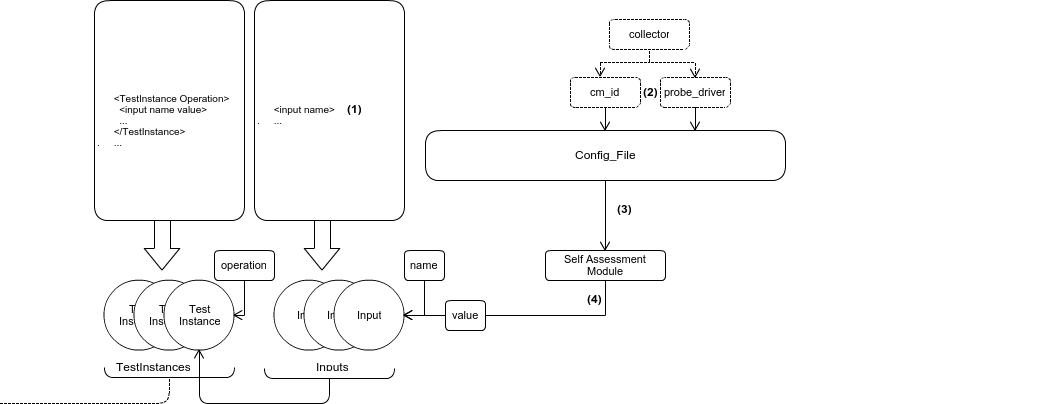
\includegraphics[width=\textwidth]{immagini/SelfAssessment.png}
}
\caption{Self Assessment Module}\label{fig:SelfAssessment}
\end{figure}
\newpage
\subsection {Probe Wrapper}
Questo componente rappresenta il punto di aggancio per un \textit{driver di sonda}.
Si occupa innanzitutto di verificare se il driver di sonda richiesto per l'esecuzione del \textit{Collector} sia disponibile e ne verifica le dipendenze. Se il driver non è presente, ne effettua il download da un repository centralizzato ed installa tutte le dipendenze dai repository del sistema operativo.
Successivamente viene effettuato un controllo di integrità del driver per individuare eventuali manomissioni.
Il driver viene poi caricato sulla sonda e ne viene lanciata l'esecuzione su tutti i TestCase.
\begin{figure}[H]
\centering
\makebox[\textwidth]{
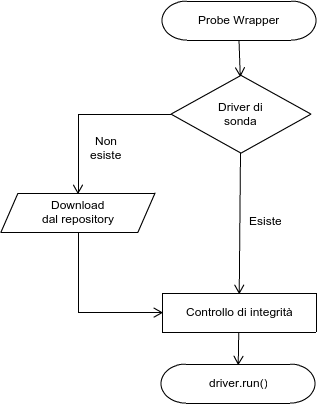
\includegraphics[width=10cm]{immagini/ProbeWrapper.png}
}
\caption{Funzionamento del Probe Wrapper}\label{fig:ProbeWrapper}
\end{figure}
\newpage
\subsection {Driver di sonda (Probe Driver)}
Il probe driver $P$, o \textit{driver di sonda}, è l'implementazione effettiva del singolo test.
Esso è strutturato da
\begin{itemize}
\item una sequenza di $n$ operazioni atomiche, con corrispondenza biunivoca con gli elementi TestInstances, che forniscono i dati in input per l'esecuzione del test.
\begin{align*}
A = \{ o_0, o_1, o_2, ... , o_n \}
\end{align*}
\item una sequenza di $n$ operazioni di rollback - una per ogni operazione atomica - che svolgono azioni di \textit{undo}
\begin{align*}
R = \lnot A = \{ r_0, r_1, r_2, ... , r_n \}
\end{align*}
\end{itemize}
aggregati in coppie ordinate
\begin{align*}
P = \{ (o_0, r_0), (o_1, r_1) , (o_2, r_2) , ... , (o_n, r_n)\}
\end{align*}
Ogni operazione atomica $o_x \in A$ riceve in input gli output dell'operazione $o_{x-1}$; analogamente ogni operazione $r_x$ di rollback $r \in R$ riceve in input gli output di $r_{x+1}$.

\begin{align*}
R_1 \subseteq R =\{ r_{x-1}, r_(x-2), ... , r_{x-n}\}
\end{align*}
e il risultato del test sarà False (2).
\begin{figure}[H]
 \begin{minipage}[b]{6cm}
   \centering
   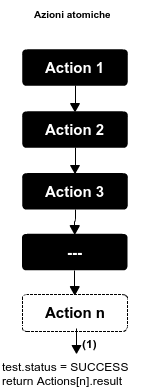
\includegraphics[width=4cm]{immagini/FlowchartProbeOk.png}
   \caption{Esecuzione corretta di un test}\label{fig:probeOk}
 \end{minipage}
 \ \hspace{2mm} \hspace{3mm} \
 \begin{minipage}[b]{9cm}
  \centering
   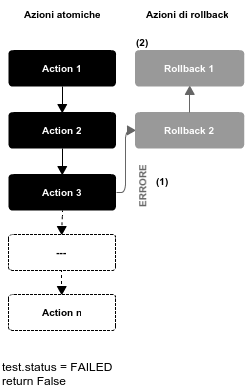
\includegraphics[width=6.6cm]{immagini/FlowchartProbeRollback.png}
   \caption{Esecuzione di un test con operazioni di rollback}\label{fig:probeRb}
 \end{minipage}
\end{figure}
Nella figura \ref{fig:probeOk} è mostrata l'esecuzione di un driver di sonda il cui test viene eseguito correttamente.
Il risultato dell'ultima operazione atomica deve essere un valore \textit{boolean} e viene utilizzato come risultato finale per tutto il test (1).

In caso di fallimento di un'operazione $o_x \in P$ , $x \leq n$ (figura \ref{fig:probeRb}) (1) l'interfaccia del Probe Driver si occupa di lasciare il sistema in uno stato sicuro provvedendo ad eseguire in sequenza le operazioni di rollback.

\subsection {Evidence Collector}
Questo componente fornisce un metodo per la raccolta delle evidenze e dei log da usare a supporto del processo di certificazione e da includere nel certificato finale.
Sono previste due modalità d'uso:
\begin{itemize}
\item Evidenze raccolte e memorizzate localmente.
\item Evidenze raccolte in modo centralizzato.
\end{itemize}

\subsection {Results Handler}
Effettua il collezionamento dei risultati dei vari TestCase e li invia al Test Manager per la valutazione.

\subsection {Monitoring Service}
Offre la possibilità di effettuare il monitoraggio della sonda. Fornisce un'interfaccia pubblica per il recupero di:
\begin{itemize}
\item informazioni di stato
\item dettagli sui test eseguiti
\item esiti e risultati dei test
\end{itemize}
\vfill
\newpage
\section{Flusso di esecuzione}
Di seguito viene riassunto il flusso di esecuzione delle operazioni sopra descritte.
\begin{figure}[H]
\centering
\makebox[\textwidth]{
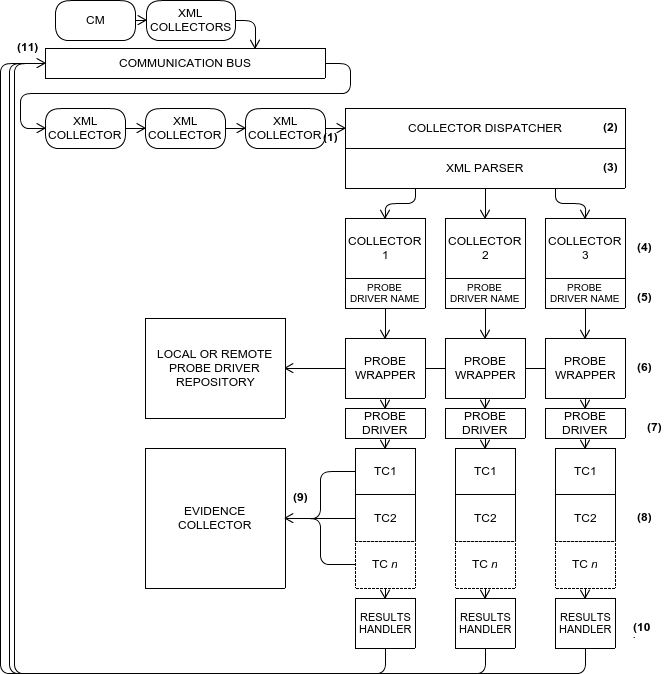
\includegraphics[width=\textwidth]{immagini/ExecutionFlow.png}
}
\caption{Flusso di esecuzione}\label{fig:ExecutionFlow}
\end{figure}
(1) Vengono ricevuti i \textit{Collector} in formato XML sul canale di comunicazione e vengono inoltrati al \textit{Collector Dispatcher} che ne prepara l'esecuzione in parallelo.
Viene poi effettuato il \textit{parsing} (3) e il \textit{marshalling} (4) dei \textit{Collector}, il probe wrapper (6) effettua i controlli sulla presenza dei driver di sonda in un \textit{repository} locale, ed eventualmente li scarica da un \textit{repository} remoto (7), effettuando controlli di integrità.
I \textit{Collector} vengono eseguiti in modo parallelo, serializzando i \textit{TestCase} (8). Durante l'esecuzione dei TestCase si possono memorizzare le evidenze tramite l'\textit{Evidence Collector} (9). I risultati vengono gestiti poi dal \textit{Results Handler} (10) e inviati nuovamente al \textit{Test Manager} tramite il canale di comunicazione (11)

\section{Valutazione dei costi}
Uno degli aspetti più critici della certificazione è rappresentato dai costi e dall'invasività che essa comporta, in relazione ai reali benefici e al valore aggiunto che offre.
La validità di un certificato, infatti, si basa principalmente sulla credibilità dell'autorità che lo ha emesso, tenendo conto degli strumenti utilizzati, dell'accuratezza con cui è stata effettuata la validazione del prodotto. e dell'affidabilità dell'intero processo di certificazione nel tempo.

Il primo costo da affrontare è dunque dato dalla \textit{Certification Authority}, che si occupa di emettere e gestire il certificato.
Sulla base di quanto affermato, è chiaro che questo costo deriva direttamente dalla credibilità della \textit{Certification Authority} stessa, la quale deve allestire un laboratorio idoneo al processo di certificazione e sottoscrivere gli standard riconosciuti nella relativa area geografica di competenza (es. ISO, IEC, IEEE, NIST, etc.).

A ciò va poi aggiunto il costo di deployment del framework di certificazione descritto, in tutti i suoi componenti.
L'attività di \textit{testing} su cui si basa il framework è generalmente considerata invasiva, specialmente per sistemi in produzione.
L'utilizzo di componenti basati sul monitoraggio (che deduce l'evento da una serie di precursori e indicatori), invece, è senza dubbio meno invasivo ma offre meno dinamicità nel processo di certificazione.

Oltre al discorso meramente economico, quindi, un framework di certificazione basato sul testing potrebbe introdurre ulteriori problematiche, più difficili da identificare, che potrebbero tradursi in danni monetari in un momento successivo difficilmente identificabile.

Alcuni test, ad esempio, potrebbero danneggiare la \textit{business-continuity} (es. test di performance sulla rete tramite flooding, test di performance per le operazioni di I/O in un hypervisor, test CPU-intensive), oppure aprire a vulnerabilità di sicurezza durante l'esecuzione di test o ancora causando minacce alla confidenzialità dei dati sensibili (es. password nei file di configurazione o nei Certification Model Instance).

Molte di queste problematiche possono essere risolte effettuando il \textit{deployment} del framework su un ambiente separato compatibile con il sistema da certificare.
Ciò comporta, ovviamente, ulteriori costi, dovuti anche all'\textit{effort} dell'\textit{accredited lab} nello stabilire l'effettiva compatibilità tra i due ambienti. 

\end{document}